\documentclass[aspectratio=169,11pt]{beamer}
\usetheme{metropolis}
\usepackage{booktabs}
\usepackage{graphicx}
\graphicspath{{../../results/figures/}}
\setbeamertemplate{frame footer}{Seeing Through the Shake}
\setbeamerfont{footnote}{size=\tiny}
\newcommand{\hl}[1]{\textcolor{orange!80!black}{\textbf{#1}}}

\title{Seeing Through the Shake}
\subtitle{Text-aware PSF estimation for blind motion deblurring of license plates}
\author{Inesh Roy (2024112015) \and Maithily Gauravkumar Bhala (2024117011)}
\institute{Digital Image Processing --- course project}
\date{}

\begin{document}
\maketitle

% ------------------------------------------------------------------
\begin{frame}{The problem}
\begin{columns}[T]
\column{0.55\textwidth}
\begin{itemize}
  \item Classical blind deblurring reads the blur off the image's own spectrum:
        \textbf{Radon} (angle) + \textbf{cepstrum} (length) + \textbf{Richardson--Lucy}.
  \item No training data, every step inspectable --- but developed and tested on texture-rich photographs.
  \item License plates are small, low-contrast, few strokes, resampled and compressed.
  \item A wrong PSF does not just fail --- it makes the plate \hl{less} legible.
\end{itemize}
\column{0.45\textwidth}
\small\textbf{Proposal objectives}
\begin{enumerate}
  \item[O1] core pipeline, validated on known kernels
  \item[O2] angle $\times$ length $\times$ noise sweep: natural vs.\ text/plates
  \item[O3] text-aware pre-processing on the same sweep
  \item[O4] confidence gate: harm avoided vs.\ good withheld
  \item[O5] real plates, OCR before/after vs.\ baseline
\end{enumerate}
\end{columns}
\end{frame}

% ------------------------------------------------------------------
\begin{frame}{How the blur is read off the spectrum}
\centering
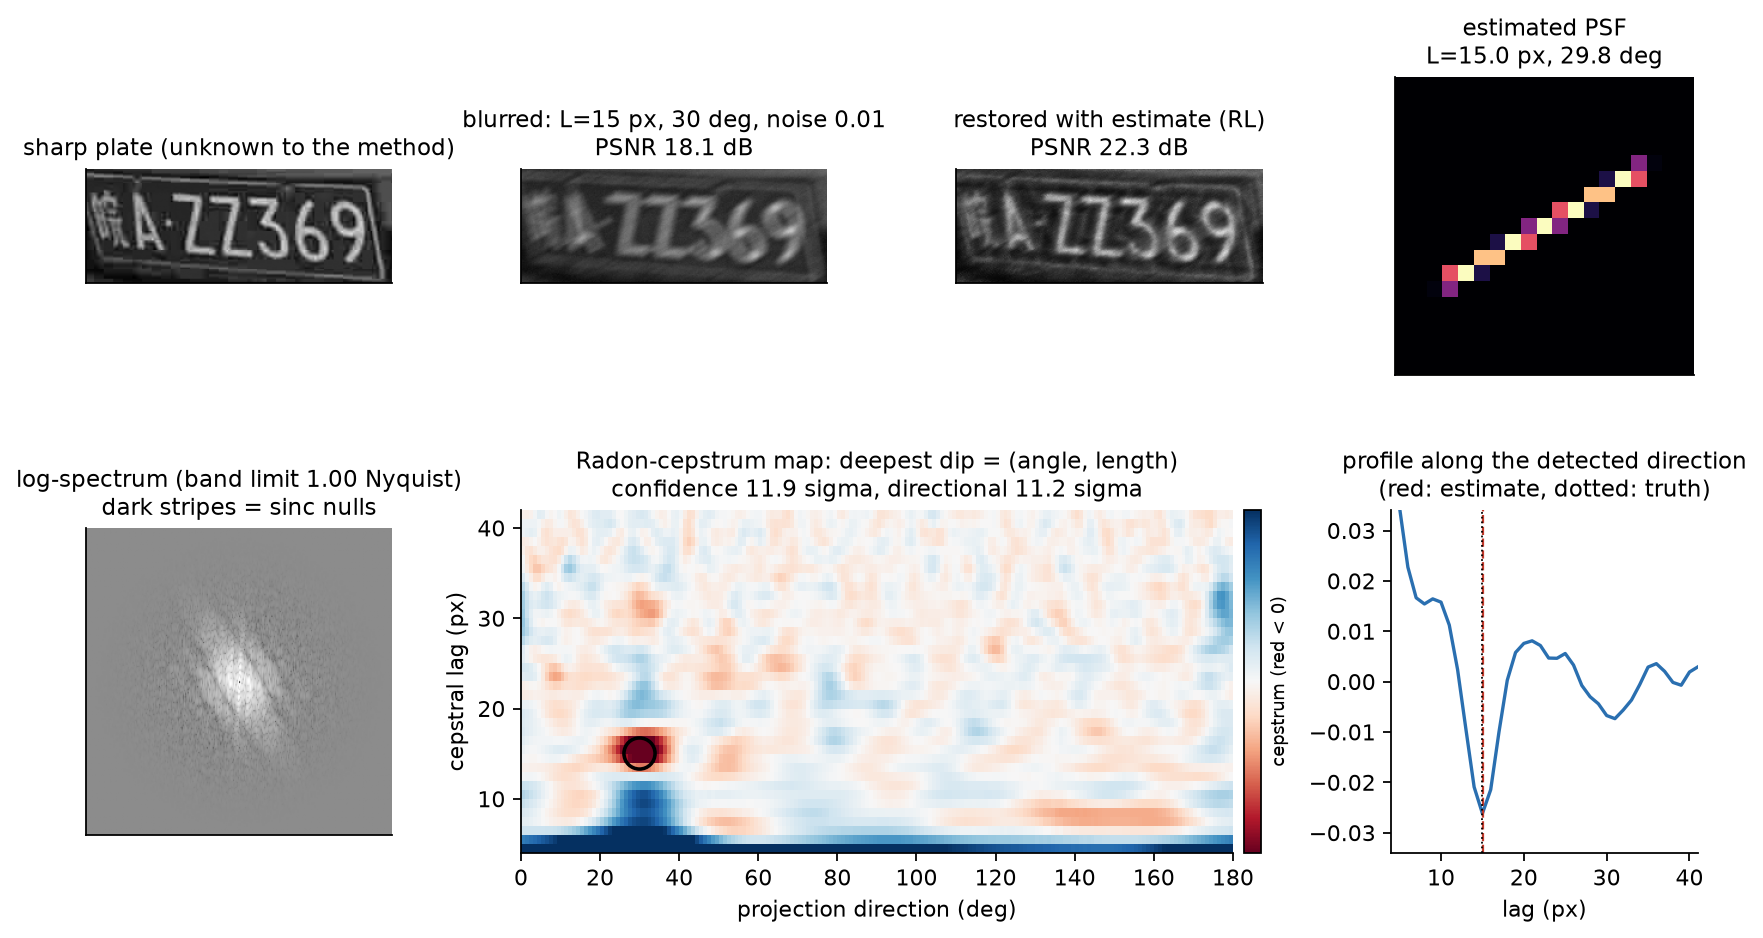
\includegraphics[width=0.93\textwidth]{07_worked_example.png}
\vspace{-2pt}
{\footnotesize Line PSF $\Rightarrow$ sinc nulls $\perp$ motion, spaced $1/L$. Radon projections of the
log-spectrum $\rightarrow$ 1-D FFT = radial cepstrum slices. Deepest negative dip $=(\theta, L)$, searched jointly.}
\end{frame}

% ------------------------------------------------------------------
\begin{frame}{Pipeline}
\begin{enumerate}
  \item Windowed log-spectrum on a square isotropic grid ($\ge 256^2$).
  \item \textbf{Joint} Radon--cepstrum search over (direction, lag), sub-degree / sub-pixel refinement.
        \\{\small (textbook rule: angle first by Radon variance, then length --- fooled by strokes; kept as reference)}
  \item \textbf{Text-aware stage}: repeat at band limits $\{1, 0.5, 0.3\}$ Nyquist, keep the most directional dip.
  \item \textbf{Gate}: dip depth $\ge 3\sigma$ \emph{and} $\ge 2$ of 4 image halves reproduce the estimate
        $\Rightarrow$ otherwise refuse, return the input unchanged.
  \item Unknown-boundary Richardson--Lucy (Wiener as comparison).
\end{enumerate}
\vspace{4pt}
{\small OCR (RapidOCR, recognition only, rectified plate) is a measuring instrument, never part of the pipeline.}
\end{frame}

% ------------------------------------------------------------------
\begin{frame}{O1 --- restoration with the true PSF}
\centering
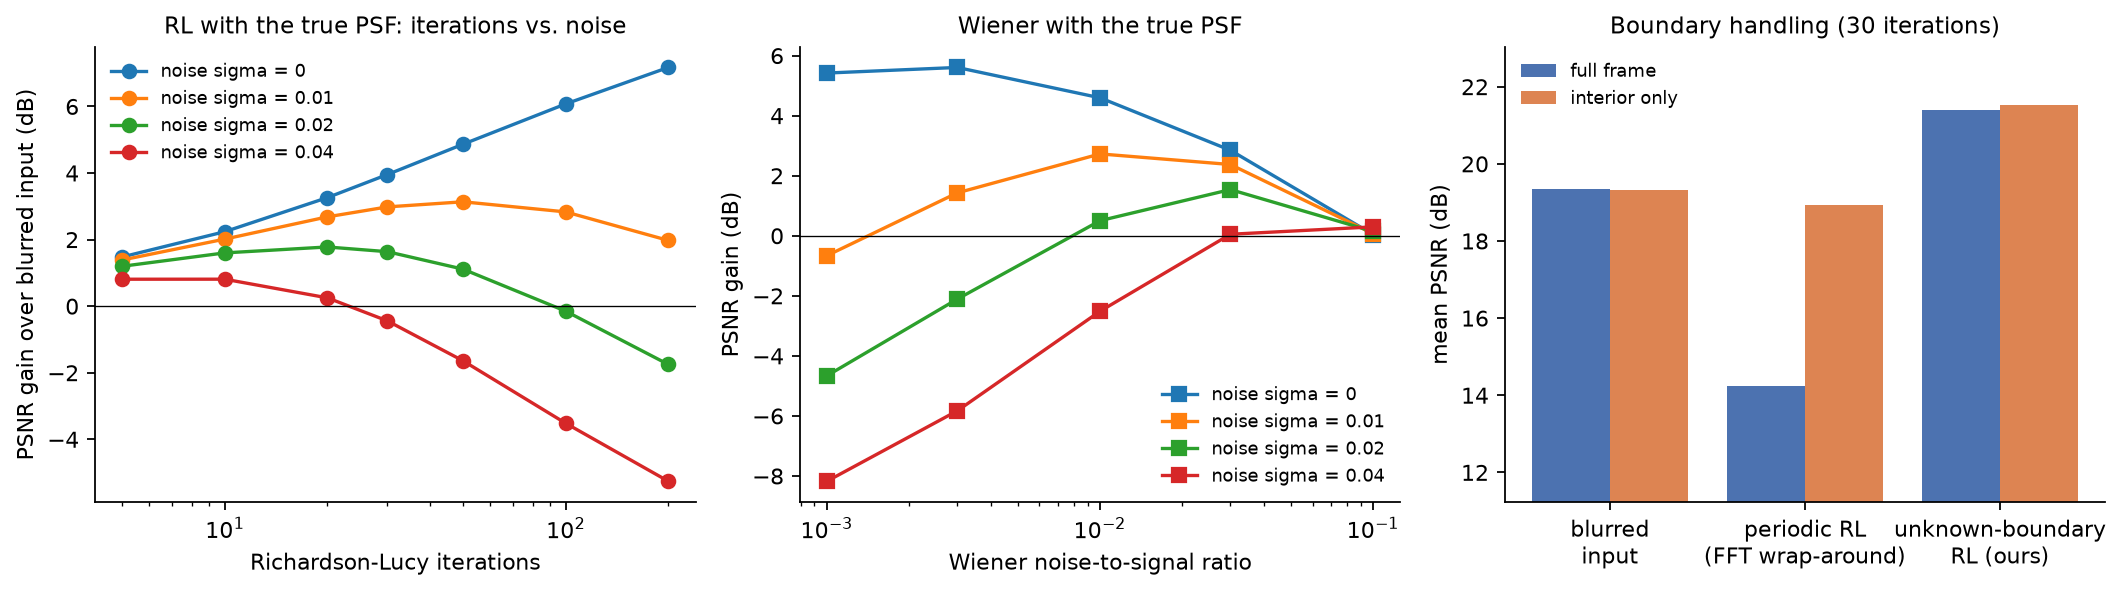
\includegraphics[width=\textwidth]{01_true_psf.png}
\begin{itemize}\small
  \item Best RL iteration count depends on noise $\Rightarrow$ discrepancy-principle stopping.
  \item Periodic RL rings at the borders; unknown-boundary RL fixes it.
\end{itemize}
\end{frame}

%RESULTS-SLIDES%

\end{document}
